% !BIB TS-program = 
\documentclass{beamer}
%\usepackage[utf8]{inputenc}
\usepackage[T1]{fontenc}
\usepackage[english,brazilian]{babel}
\usetheme{Luebeck}
\usepackage{graphicx}
\usepackage{hologo}
\usepackage{outlines}
\usepackage{listings}
%\usepackage{verbatim}
%\usecolortheme{beaver}
\mode<presentation>
\setbeamertemplate{page number in head/foot}[totalpagenumber]
\AtBeginSection[]
{
  \begin{frame}
    \frametitle{Onde Estamos?}
    \tableofcontents[currentsection,hideallsubsections ]
  \end{frame}
}



\title{Processando Texto}
\subtitle{Seminário \LaTeX - Parte I}


\author{Geraldo Xexéo\inst{1,2}}

\institute[DCC/PESC]{\inst{1}Departamento de Ciências da Computação 
\and
\inst{2}Programa de Engenharia de Sistemas e Computação}

\date[LUDES/LINE]{3o Seminário LUDES/LINE, Março 2020}



\begin{document}


\begin{frame}
\titlepage
\centering
%
\includegraphics[width=.6\linewidth]{Images/Logomarcas.png}
\end{frame}

\begin{frame}
\frametitle{Agenda}
\tableofcontents[hideallsubsections]
\end{frame}


\section{A Cadeia de Processamento de Texto}



\subsection{A Cadeia de Processamento de Texto}
\begin{frame}{A Cadeia de Processamento de Texto}
    \begin{center}
        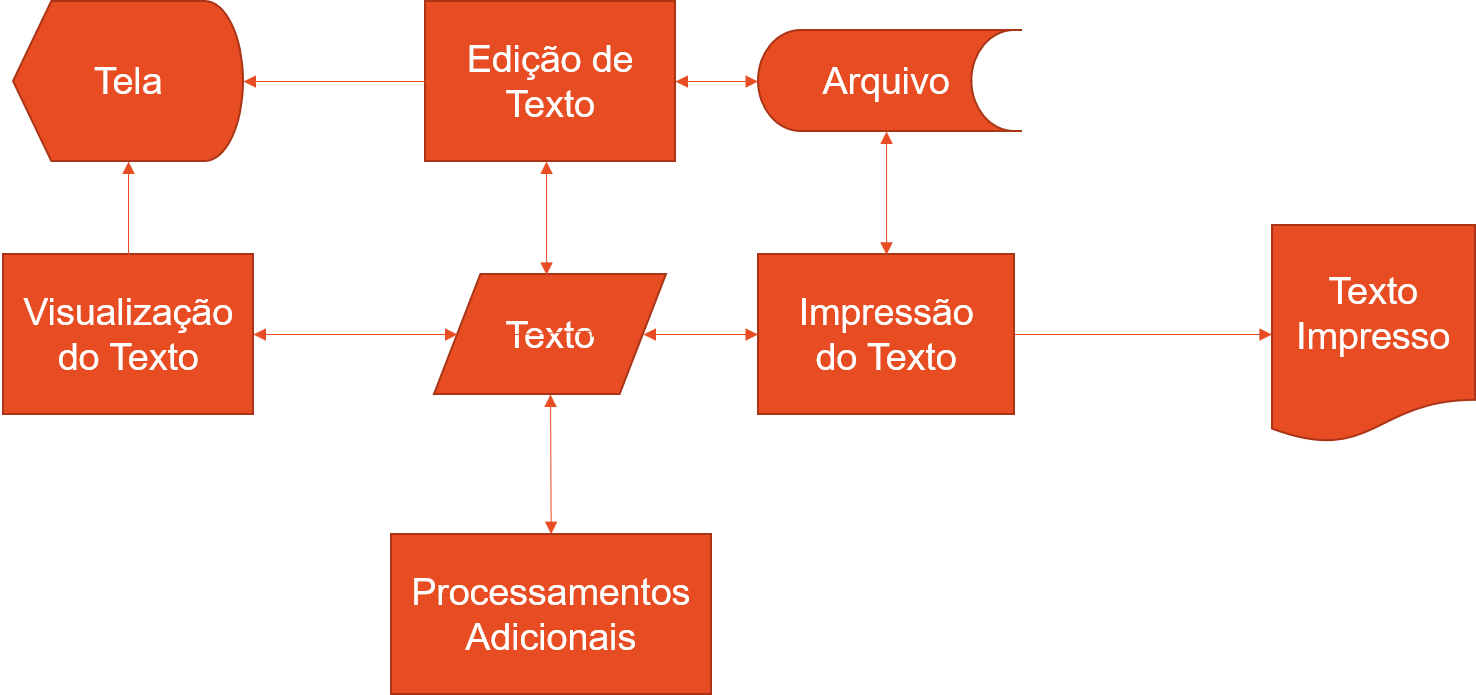
\includegraphics[width=0.7\linewidth]{Images/cadeia}
    \end{center}
    
\end{frame}

\subsection{Tipos de Sistemas}
\begin{frame}[shrink=10]{Tipos de Sistemas}
    \begin{columns}
        \begin{column}{0.5\textwidth}
            \begin{outline}
                \1 <1-> Editor de Texto
                \2 <2-> vi, \textbf{vim}, Emacs, TextEditor, Notepad++
                \1 <3-> Ambientes Integrados de Desenvolvimento (IDE)      
                \2 <4-> \textbf{\TeX Studio}, Visual Studio
                \1 <5-> Processador de Texto 
                \2 <6-> \textbf{Word}
                \1 <7-> Sistemas de Autoria
                \2 <7-> Scrivener
                \1 <8-> Desktop Publishing
                \2 <8-> Framemaker
                \1 <9-> \LaTeX\
                \1 <11-> Sistemas Colaborativos de Edição
                \2 <11-> Overleaf
            \end{outline}
        \end{column}
        \begin{column}{0.5\textwidth}
            \begin{figure}
                \begin{overprint}
                    \onslide<1>
                        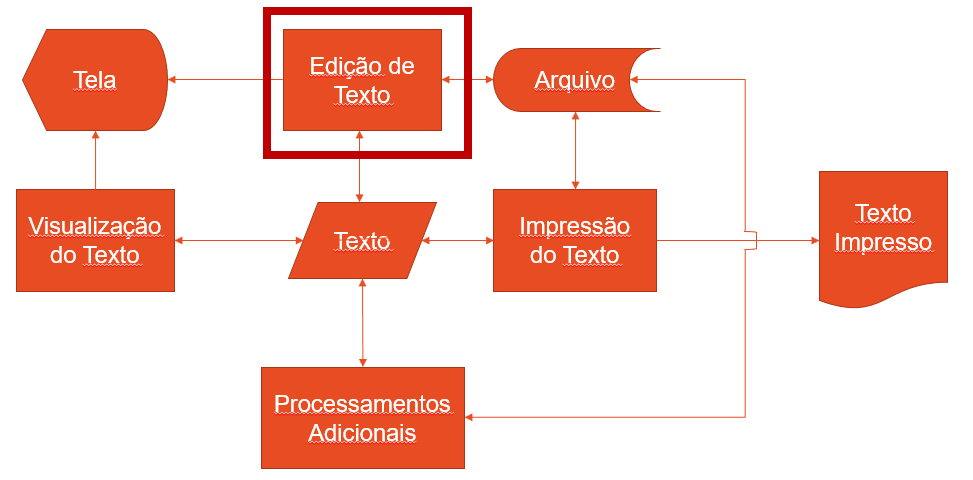
\includegraphics[width=0.8\linewidth]{Images/editordetexto.png}
                    \onslide<2>
                        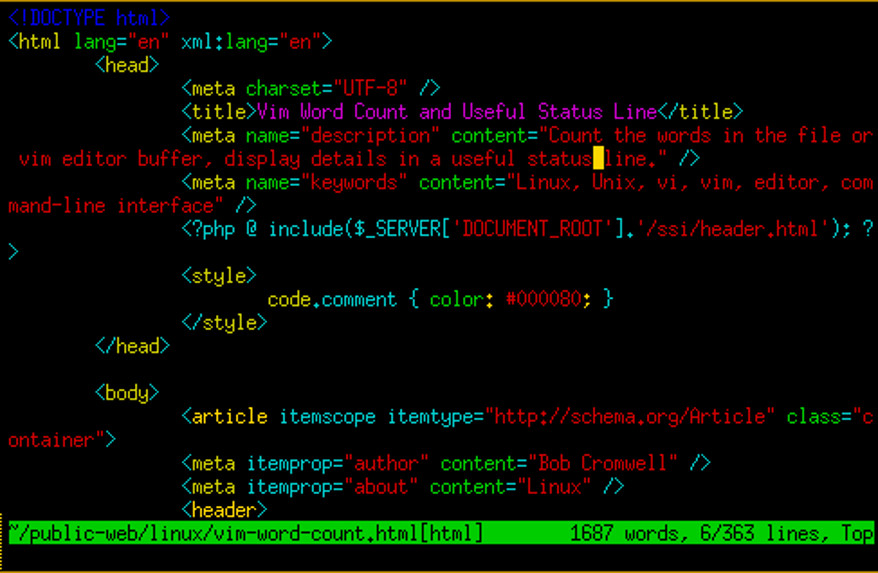
\includegraphics[width=0.8\linewidth]{Images/vim.png}     
                    \onslide<3>
                        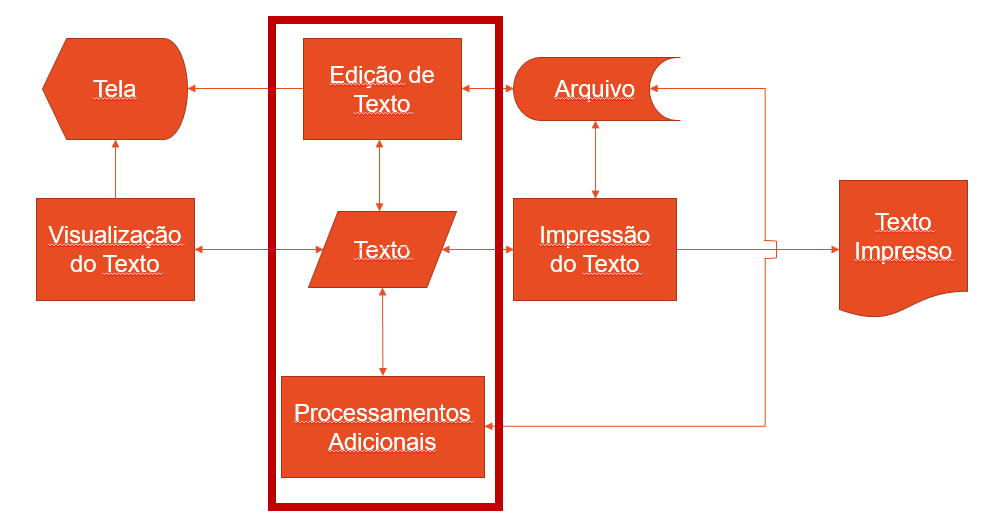
\includegraphics[width=0.8\linewidth]{Images/ide.png}
                    \onslide<4>
                        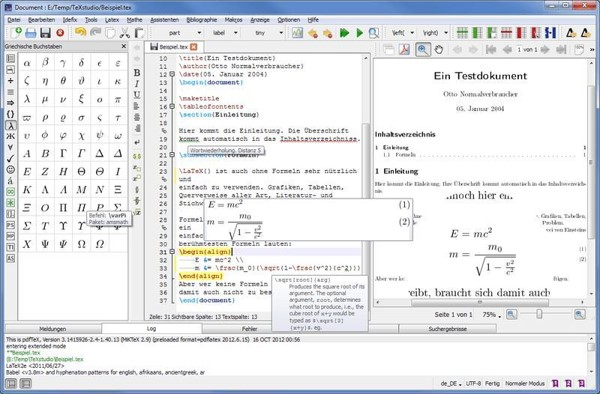
\includegraphics[width=0.8\linewidth]{Images/texstudio.jpg}    
                    \onslide<5>
                        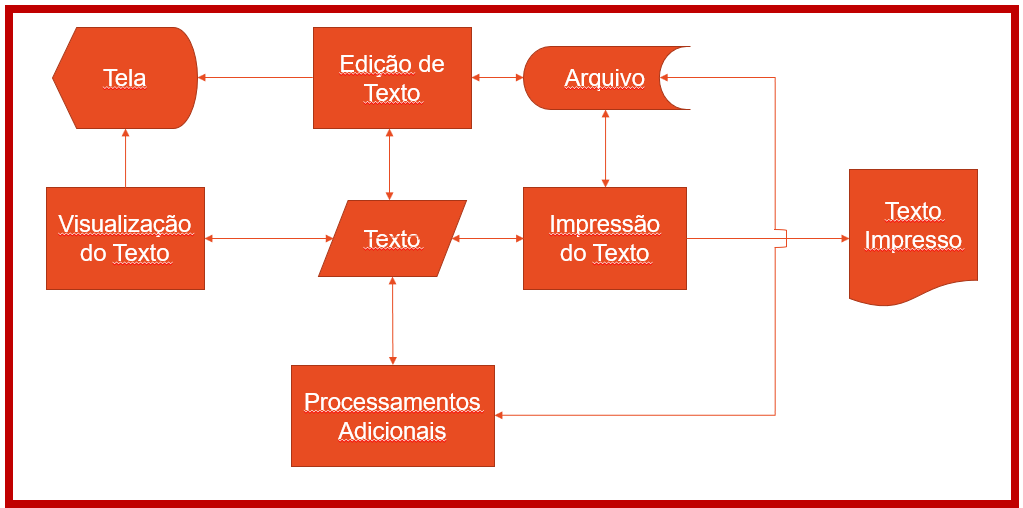
\includegraphics[width=0.8\linewidth]{Images/processador.png}    
                    \onslide<6>
                        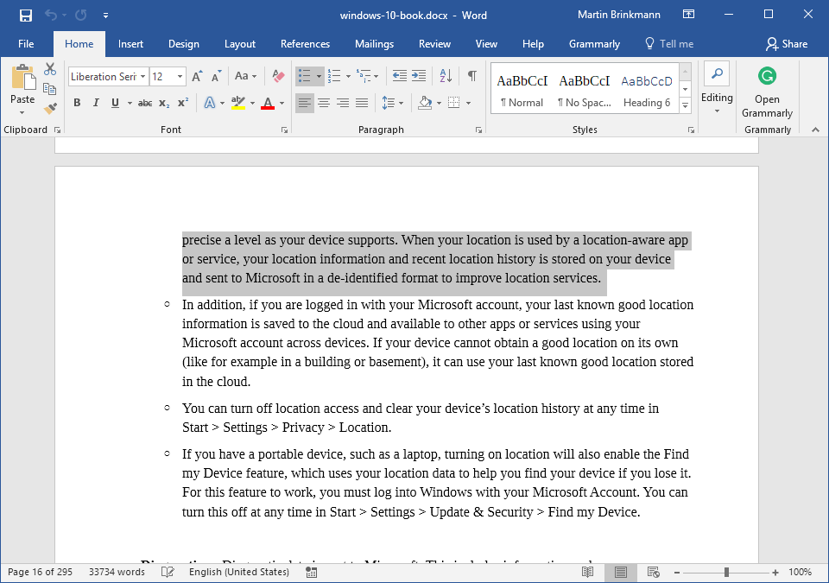
\includegraphics[width=0.8\linewidth]{Images/word.png}    
                    \onslide<7>
                        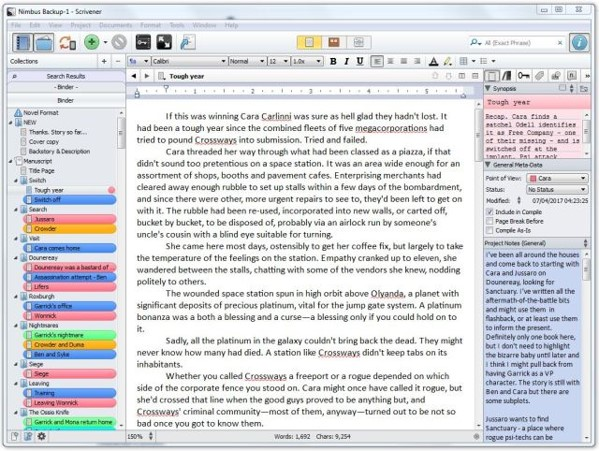
\includegraphics[width=0.8\linewidth]{Images/scrivener.jpg}    
                    \onslide<8>
                        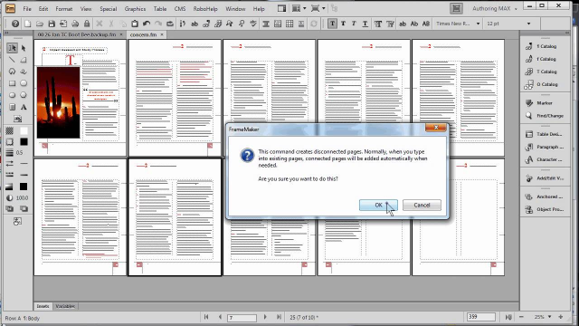
\includegraphics[width=0.8\linewidth]{Images/framemaker.png}    
                    \onslide<9>
                        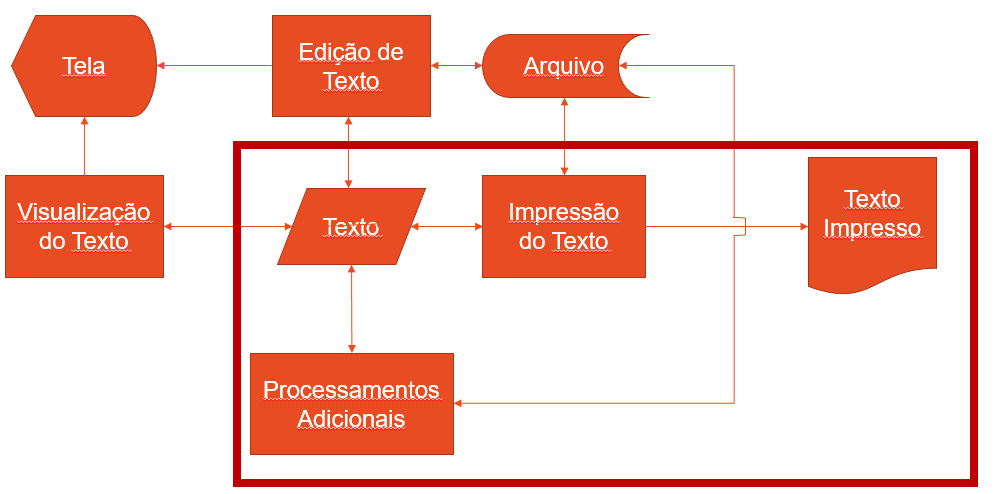
\includegraphics[width=0.8\linewidth]{Images/latex1.png}    
                    \onslide<10>
                        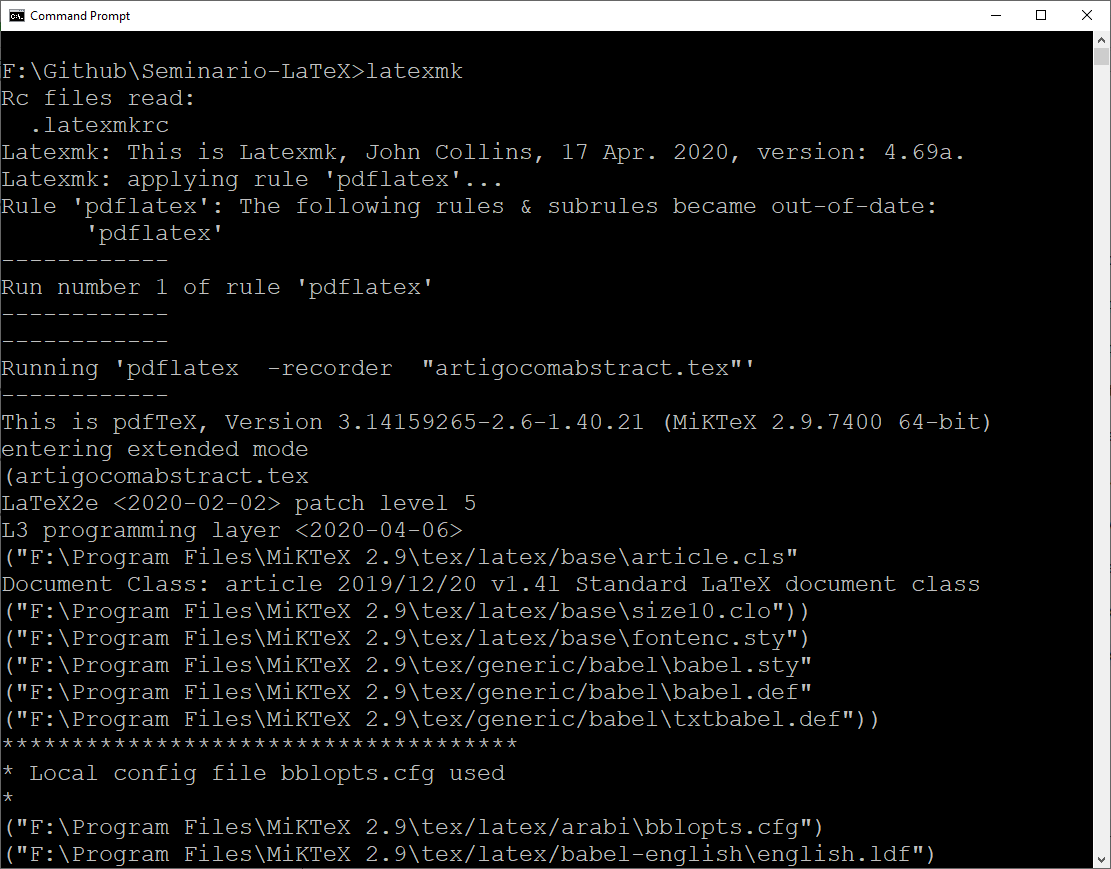
\includegraphics[width=0.8\linewidth]{Images/latex2.png}     
                    \onslide<11>
                        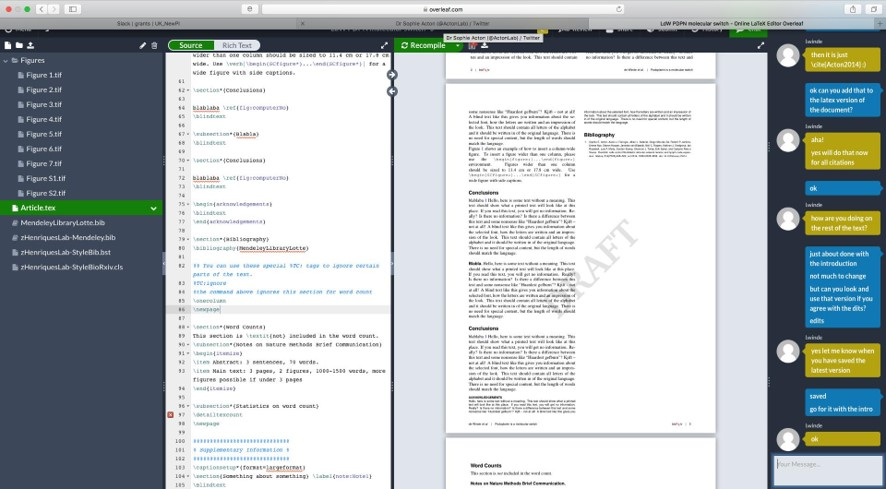
\includegraphics[width=0.8\linewidth]{Images/overleaf.jpg}                                                         
                \end{overprint}
            \end{figure}
        \end{column}
    \end{columns}
\end{frame}

\subsection{Tipos de Linguagens}
\begin{frame}{Tipos de Linguagens}
    \begin{columns}
        \begin{column}{0.5\textwidth}
            \begin{outline}
                \1 <1-> Linguagens de Impressão/Visualização
                \2 <1-> PostScript, DVI, PDF 
                \2 <1-> Você quase não mexe
                \1 <2-> Linguagens de Marcação      
                \2 <2-> SGML, HTML, \TeX\, \LaTeX\, Markdown, RPF, fods
                \1 <3-> Linguagens Intermediárias 
                \2 <3-> .dvi
                \2 <3-> Você não mexe
            \end{outline}
        \end{column}
        \begin{column}{0.5\textwidth}
            \begin{figure}
                \begin{overprint}
                    \onslide<1>
                    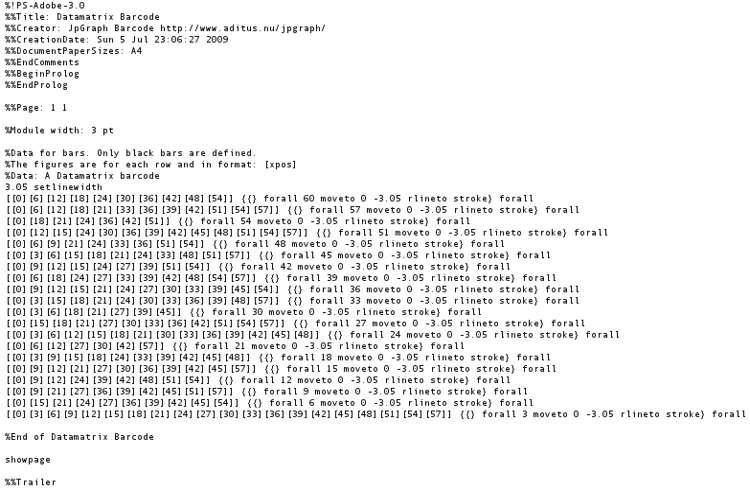
\includegraphics[width=0.8\linewidth]{Images/ps.png}
                    \onslide<2>
                    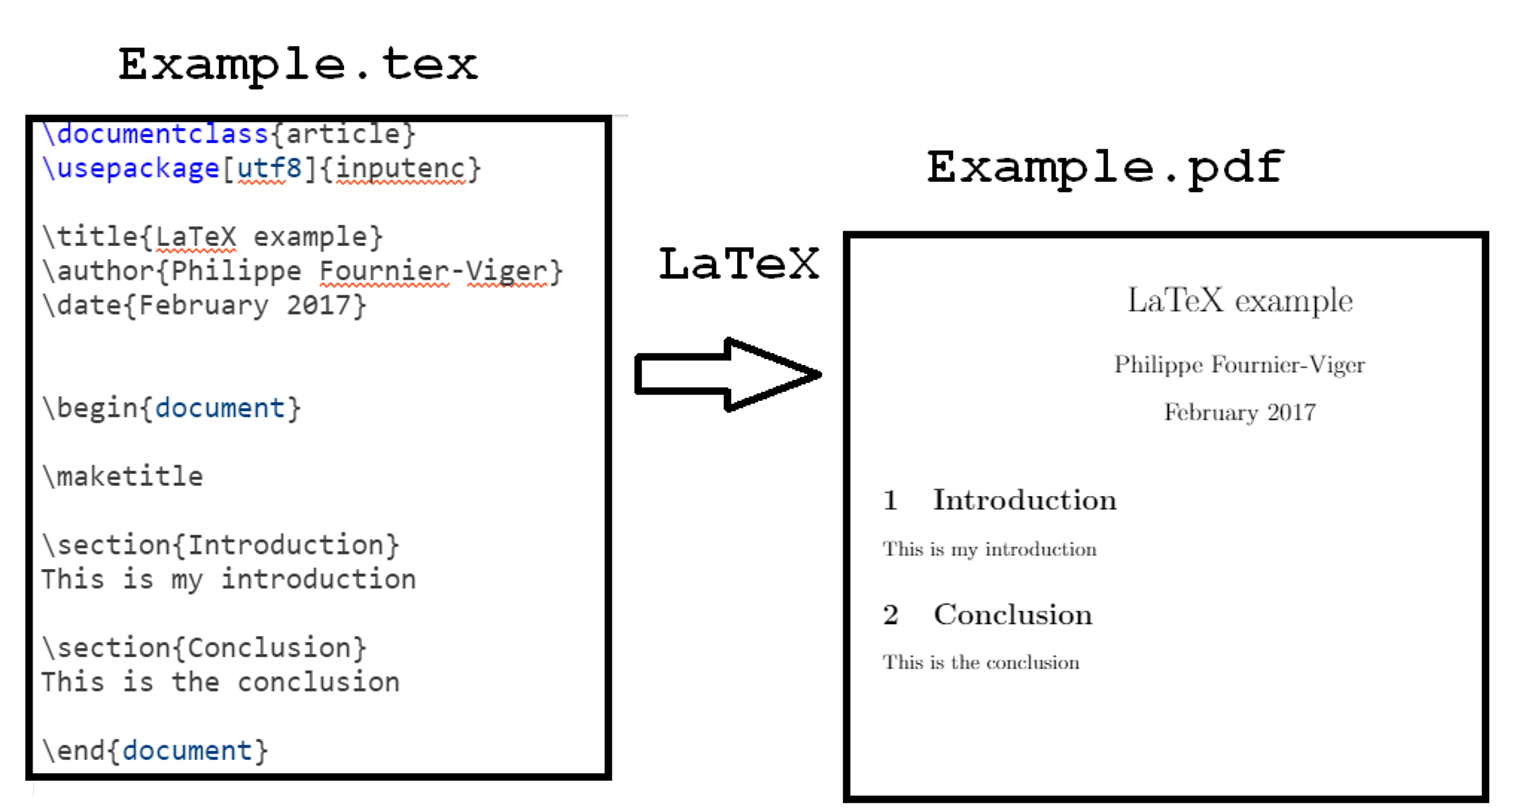
\includegraphics[width=0.8\linewidth]{Images/marcacao.png}                                          
                \end{overprint}
            \end{figure}
        \end{column}
    \end{columns}
\end{frame}

\subsection{Sistemas Mais Usado na Computação}
\begin{frame}{Sistemas Mais Usados na Computação}
    \begin{outline}
        \1 Word
        \2 WYSIWYG
        \2 Líder do mercado
        \2 Superpoderoso
        \2 Ruim para trabalho colaborativo
        \1 Google Docs
        \2 WYSIWYG?
        \2 Sucesso nos jovens
        \2 Pouca expressão gráfica
        \2 Ótimo para trabalho colaborativo
        \1 \LaTeX\
        \2 Melhor imagem de texto, mas no detalhe
        \2 Ótimo para Matemática
        \2 Difícil de usar
        \2 Empoderado pelo Overleaf
        \3 Colaboração!
    \end{outline}
\end{frame}

\section{Mitos e Fatos}

\begin{frame}{Mitos e Fatos}
    \begin{outline}
        \1 Qualidade de saída do \LaTeX\ é muito melhor
        \2 \textbf{Sim}, é um sistema de typesetting
        \2 Cuidado, pois ele pode gerar erros graves, olhe sua saída
        \2 O pessoal do Word nem sabia o que estava fazendo
        \2 Mas... É no detalhe. E se você configurar bem.
        \1 Word não trabalha bem com fórmula
        \2 \textbf{Falso}, melhorou muito
        \2 Mas não são tão bonitas na impressão
        \1 Não consigo colocar a imagem onde quero no Word
        \2 \textbf{Falso}, e tente no \LaTeX\
        \2 Sempre tem um jeito
    \end{outline}
\end{frame}

\begin{frame}{Mitos e Fatos II }
    \begin{outline}
        \1 Você perde muito tempo com besteira no \LaTeX\
        \2 \textbf{Fato}
        \1 \LaTeX\ é mais produtivo porque você pensa não pensa no formato
        \2 \textbf{Mito}, na verdade as pesquisas mostram que \LaTeX\ é igual ou menos produtivo que Word
        \1 Em \LaTeX\ gerencio melhor as bibliografias
        \2 \textbf{Mito}, sistemas como Zotero são equivalentes
        \1 Em \LaTeX\ consigo controlar versões
        \2 \textbf{Fato}, mas aprendemos um truque do Word+pandoc+Git!
    \end{outline}
\end{frame}

\begin{frame}{Mitos e Fatos III }
    \begin{outline}
        \1 Word é mais fácil de aprender
        \2 \textbf{Fato}
        \1 Basta o Word
        \2 \textbf{Mito}, você precisa de, no mínimo, gerenciar arquivos e usar um sistema de biblografia
        \1 Word tem problemas com arquivos grandes
        \2 Acontece de verdade, é melhor não usar 
    \end{outline}
\end{frame}

\section{Recomendações}
\begin{frame}[shrink=20]{Recomendações}
    \begin{columns}
        \begin{column}{0.5\linewidth}
            \begin{outline}
                \1 Word
                    \2 Ótima para 1 escritor principal e 1 revisor
                    \2 Arquivos pequenos a grandes, mas cuidado com os muito grandes
                        \3 Divida sempre em capítulos para editar e junte para imprimir
                        \3 Master Document está bugado há muito tempo
                    \2 Faça o seu backup
                        \3 Me pergunte sobre o Git depois
                \1 Google Docs
                    \2 Ótimo para muitas pessoas
                    \2 Sem controle de quem faz o que
                    \2 Não é bom para formatação 
                        \3 Passe para o Word no final
                    \2 Aquivos pequenos
                        \3 Backup automático     
           \end{outline}     
        \end{column}
        \begin{column}{0.5\linewidth}
            \begin{outline}
            \1 \LaTeX
                \2 Se a editora fornece o formato, é a melhor opção
                \2 Para a Tese na Coppe, é ótima opção
                    \3 Use o JabRef, ou o Zotero e o JabRef
                \2 Overleaf
                    \3 Bom para artigos de poucas pessoas
                    \3 Pode ter dificuldades com uma tese
                    \3 Ligue as opções de Github, Dropbox, etc. (Backup!)
                \2 Em casa
                    \3 Use o Git+Nuvem
                    \3 Mantenha a instalação atualizada!
                    \3 Faça backup, faça backup, faça backup
                \end{outline}
        \end{column}
    \end{columns}
\end{frame}


\begin{frame}
\Huge \center
Obrigado!
\end{frame} 

\begin{frame}{Contato}
\begin{center}
    
\includegraphics[width=\linewidth]{Images/Picture5.png}
\end{center}   
\end{frame}

\end{document}
